\documentclass[11pt, oneside]{article}   	% use "amsart" instead of "article" for AMSLaTeX format
\usepackage{geometry}                		% See geometry.pdf to learn the layout options. There are lots.
\geometry{letterpaper}                   		% ... or a4paper or a5paper or ... 
%\geometry{landscape}                		% Activate for for rotated page geometry
%\usepackage[parfill]{parskip}    		% Activate to begin paragraphs with an empty line rather than an indent
\usepackage{graphicx}				% Use pdf, png, jpg, or eps� with pdflatex; use eps in DVI mode
								% TeX will automatically convert eps --> pdf in pdflatex		
\usepackage{amssymb}
\usepackage{amsmath}
\usepackage{parskip}
\usepackage{url}

\title{Public Key Cryptography:  example}
%\author{The Author}
\date{}							% Activate to display a given date or no date
\graphicspath{{/Users/telliott_admin/Dropbox/Tex/png/}}

\begin{document}
\maketitle
%\section{}
%\subsection{}
\Large
In this short write-up we will go through an example of using public-key cryptography.   Let's explore a simple example of file encryption using \texttt{ssh} and \texttt{openssl}.  The demo uses OS X Terminal but it would be very similar on Linux.

The first step is to generate an RSA key pair.  Normally one would do something like:

\texttt{ssh-keygen -t rsa -C "name@host"}

where -C is a comment (for convenience of the user only, not transmitted), -t is the type of key, -b is number of bits (the default for RSA is 2048), and -m is the format (the default is RFC4716 but PEM is also an option).

Since I am not currently using RSA keys, I could just write them to the default filepaths:  \texttt{\textasciitilde /.ssh/id\_rsa} and \texttt{\textasciitilde /.ssh/id\_rsa.pub} .

Instead, for this demo I'm going to put them on the Desktop:

\texttt{ssh-keygen -t rsa -C "te" -f ./kf}

At the prompt, I enter a passphrase:  \texttt{abcde}

The output is:

\begin{center} 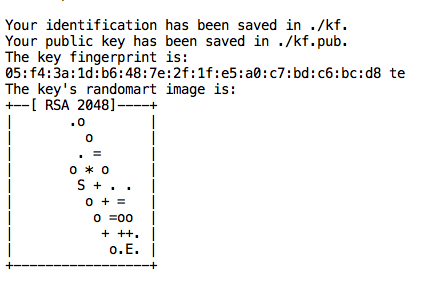
\includegraphics [scale=0.75] {rsa.png} \end{center}

There are two files:  \texttt{kf} and  \texttt{kf.pub}.  We can check the fingerprint like this:

\texttt{ssh-keygen -lf kf}

The output is:

\texttt{2048 05:f4:3a:1d:b6:48:7e:2f:1f:e5:a0:c7:bd:c6:bc:d8  te (RSA)}

Now for an example:

\texttt{echo "hello world" > \textasciitilde /Desktop/p.txt}

The next step uses \texttt{openssl}.  It can do a lot of things, for example, digests.  Here are some approaches

\texttt{echo "hello world" | openssl sha1 \\
echo "hello world" | openssl md5 \\
openssl md5 ./p.txt} 

I'm having trouble typesetting the output, but you can check it out in this screenshot:

\begin{center} 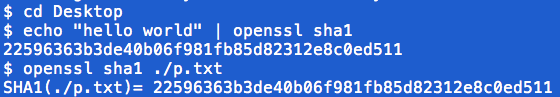
\includegraphics [scale=0.75] {rsa3.png} \end{center}

\texttt{openssl} can also do base64 encoding:

\texttt{openssl base64 -in p.txt -out b.txt \\
openssl base64 -d -in b.txt}

\url{en.wikipedia.org/wiki/Base64}

We first use it to re-format the public key as PEM:

\texttt{openssl rsa -in kf -pubout > ./kf.pem}

Now we can write this short message:

\texttt{echo "hello world" > ~/Desktop/p.txt}

Encrypt

\texttt{cat p.txt | openssl rsautl -encrypt \textbackslash \\
-pubin -inkey kf.pem > c.txt}

The \texttt{-pubin} option means to encrypt with the public key
We can also specify the input and output files like this:

\texttt{openssl rsautl -encrypt -in p.txt  \textbackslash \\
-out c.txt -pubin -inkey kf.pem}

Take a look

\texttt{hexdump -C c.txt}

\begin{center} 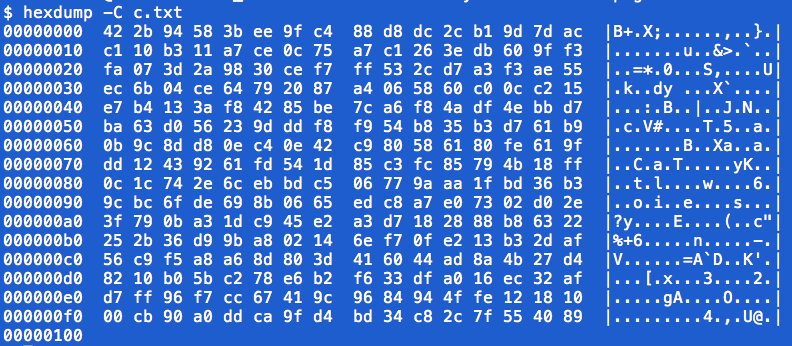
\includegraphics [scale=0.5] {rsa2.png} \end{center}

Decrypt with the private key

\texttt{\$ openssl rsautl -decrypt -in c.txt -inkey kf \\
Enter pass phrase for kf: \\
hello world}

We can use the keys the other way around, encrypting with the private key and decrypting with the public one:

The options are \texttt{-sign} and \texttt{-verify}

\texttt{openssl rsautl -sign -in p.txt -out c.txt -inkey kf \\
openssl rsautl -verify -in c.txt -pubin -inkey kf.pem}

\subsection*{}

With a larger message to encrypt, we have to be more sophisticated

\url{www.czeskis.com/random/openssl-encrypt-file.html}

Generate 256 random bytes (the source does it in two steps, so that's what we'll do:

\texttt{openssl rand 128 > k1.bin \\
openssl rand 128 > k2.bin \\
cat k1.bin k2.bin > k.bin}

To encrypt using AES with 256 bits and CBC mode:

\texttt{openssl enc -aes-256-cbc -salt -in p.txt  \textbackslash \\
 -out c.txt -pass file:./k.bin}

To decrypt:

\texttt{openssl enc -d -aes-256-cbc -in c.txt  \textbackslash \\
 -out m.txt -pass file:./key.bin}

In practice, use the RSA key to send this key to your cohort.  You should also verify the digest (hash) of the data you send, or sign it with your private key (see above)

I have written quite a bit about the structure of RSA key files.  See:

\url{telliott99.blogspot.com/2011/08/dissecting-rsa-keys-in-python.html}

There are four posts, and I explore the use of Python modules to do encryption.

\end{document}  